\chapter{Risultati} \label{chp:risultati}
In questo capitolo verranno presentati i risultati ottenuti dalle due fasi di valutazione
delle diverse versioni dei modelli separati in base ai dataset su cui sono stati 
allenati: \texttt{dataset\_corr} e \texttt{dataset\_pca}. Prima verranno presentati
i risultati ottenuti dalla validazione $80/20$ con gli iperparametri migliori 
ottenuti nel capito precedente, successivamente verranno presentati
i risultati ottenuti dalla cross-validation.

% Prima di esporre i risultati ottenuti, è opportuno enunciare la seguente premessa.
% Considerando la natura del contesto, mirante alla classificazione di dati medici,
% si è convenuto di regolare manualmente il valore della soglia per la predizione
% del tumore. Tale decisione è stata presa al fine di minimizzare il numero di
% falsi negativi, ossia i casi in cui il modello erroneamente predice l'assenza di
% tumore quando invece è presente.

% Per effettuare questa operazione, è stato selezionato il valore di soglia pari a
% $0.3$, al fine di ridurre il numero di falsi negativi. Questa determinazione è
% stata adottata per conferire maggior rilevanza al valore di richiamo, che valuta
% l'efficacia del modello nell'individuare i veri positivi.

I classificatori sono stati valutati calcolando la matrice di confusione, successivamente
sono state calcolate le metriche associate alla matrice appena calcolata:
\begin{itemize}
    \item \textbf{Accuracy}: misura la frazione di esempi classificati correttamente.
    \item \textbf{Precision}: misura la frazione di esempi classificati come
          positivi che sono effettivamente positivi.
    \item \textbf{Recall}: misura la frazione di esempi positivi che sono stati
          classificati correttamente.
    \item \textbf{F1-score}: media armonica tra precisione e recall.
\end{itemize}
Inoltre, sono state calcolate le curve ROC per analizzare TP rate e FP rate.
Infine, per la seconda fase di validazione, dal momento che è stata effettuata una 
$10$-fold cross-validation, sono state calcolate per ciascuno dei 10 apprendimenti
le metriche di Accuracy, Precission, Recall e F1-score in modo da ottenere gli 
intervalli di confidenza, per analizzare la robustezza dei modelli 

% Nelle successive sezioni verranno esposti i risultati ottenuti per ciascun
% modello, confrontando i valori delle metriche di valutazione e le curve ROC
% generate. I risultati saranno suddivisi in due sezioni, una per il confronto
% sul dataset le cui feature sono state selezionate manualmente, una per il
% confronto sul dataset le cui feature sono state selezionate con PCA.
\section{Risultati dei modelli allenati su \texttt{dataset\_corr} e \texttt{dataset\_corr\_std}} \label{sec:risultati_corr}
Per prima cosa sono state prodotte le matrici di confusione per ciascun modello
raffigurate nella figura \ref{fig:matrice_di_confusione_per_corr}.

\textbf{TODO:confronto dei valori nelle matrici di confusione}.

Dalle matrici di confusione si possono calcolare le metriche di Accuracy, Precission, 
Recall e F1-score. Nella tabella \ref{tab:risultati} sono riportati i valori delle 
metriche di valutazione ottenutes per ciascun modello calcolate sul test set, il quale
composto dal $20\%$ di \texttt{dataset\_corr} e \texttt{dataset\_corr\_std}.
\begin{table}[!ht]
    \centering
    \begin{tabular}{@{}cllll@{}}
        \toprule
        \rowcolor[HTML]{EFEFEF}
        \textbf{Modello}                                      & \textbf{Accuratezza}         & \textbf{Precisione}          & \textbf{Richiamo}            & \textbf{F1 score}            \\ \midrule
        \cellcolor[HTML]{EFEFEF}\textbf{SVM}                  & \multicolumn{1}{c}{0 \%}     & \multicolumn{1}{c}{0 \%}     & \multicolumn{1}{c}{0 \%}     & \multicolumn{1}{c}{0 \%}     \\
        \cellcolor[HTML]{EFEFEF}\textbf{Gaussian Naive Bayes} & \multicolumn{1}{c}{95 \%}    & \multicolumn{1}{c}{90 \%}    & \multicolumn{1}{c}{99 \%}    & \multicolumn{1}{c}{94 \%}    \\
        \cellcolor[HTML]{EFEFEF}\textbf{Rete neurale}         & \multicolumn{1}{c}{98.93 \%} & \multicolumn{1}{c}{98.52 \%} & \multicolumn{1}{c}{99.10 \%} & \multicolumn{1}{c}{98.81 \%} \\ \bottomrule
    \end{tabular}
    \caption{Risultati ottenuti dal modello addestrato}
    \label{tab:risultati}
\end{table}

\textbf{TODO:controllare se è vero}
% ! Commento da riguardare e sistemare
I risultati ottenuti rivelano prestazioni superiori per i modelli basati su una
manipolazione geometrica dei dati, come la rete neurale e il Support Vector
Machine (SVM), rispetto al modello fondato su una manipolazione probabilistica,
come il Gaussian Naive Bayes.

Tale fenomeno può essere razionalizzato considerando che le distribuzioni delle
caratteristiche del dataset non rispecchiano una distribuzione gaussiana, come
supposto dal modello Gaussian Naive Bayes. Inoltre, la rete neurale e il SVM
sono modelli intrinsecamente più complessi rispetto al Gaussian Naive Bayes,
consentendo loro di catturare relazioni più intricate tra le features e
la variabile target.

In aggiunta, l'ottimo risultato osservato suggerisce una distinta separazione tra le
due classi del dataset, suggerendo che i modelli sono capaci di generalizzare
efficacemente.

\begin{figure}[!ht]
    \centering
    \begin{subfigure}{0.45\textwidth}
        \centering
        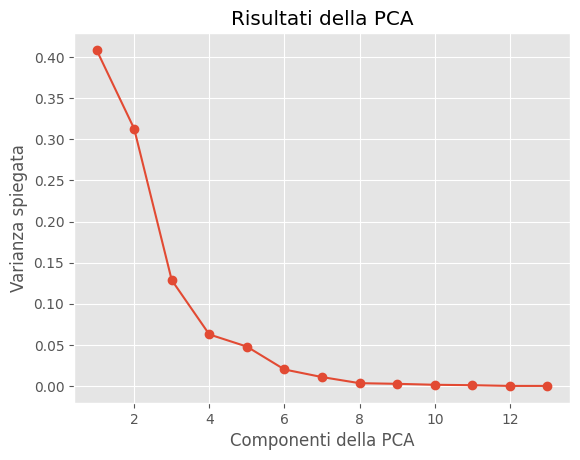
\includegraphics[width=\textwidth]{img/analisi/pcaVarianza.png}
        \caption{Support Vector Machine}
        \label{fig:matrice_di_confusione_per_SVM_corr}
    \end{subfigure}
    \hfill
    \begin{subfigure}{.45\textwidth}
        \centering
        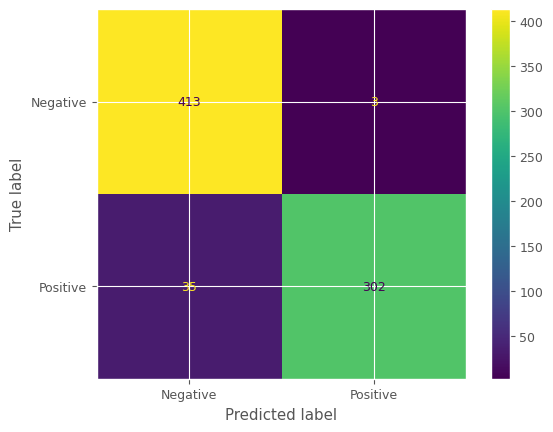
\includegraphics[width=\textwidth]{img/gnb/confusion_matrix_corr.png}
        \caption{Gaussian Naive Bayes}
        \label{fig:matrice_di_confusione_per_GNB_corr}
    \end{subfigure}
    \hfill
    \begin{subfigure}{.45\textwidth}
        \centering
        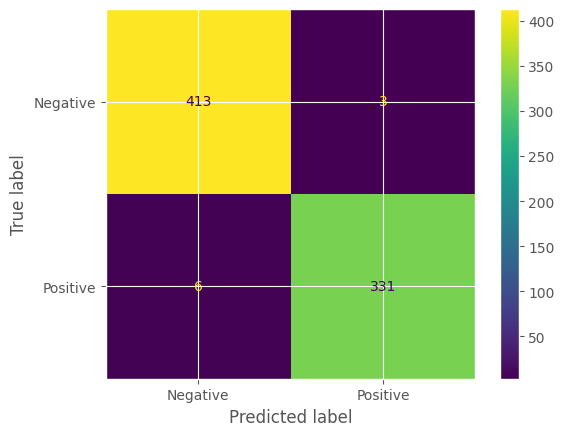
\includegraphics[width=\textwidth]{img/rete/matrice_confusione.png}
        \caption{Rete neurale}
        \label{fig:matrice_di_confusione_per_NN_corr}
    \end{subfigure}
    \caption{Matrici di confusione per i modelli addestrati su \texttt{dataset\_corr} e \texttt{dataset\_corr\_std}}
    \label{fig:matrice_di_confusione_per_corr}
\end{figure}
% TODO: Creare le immagini nuove per le matrici di confusione senza griglia

In seguito, si è deciso di confrontare i modelli utilizzando un ulteriore metrica,
ovvero AUC e le curve ROC, le quali permettono di confrontare i modelli in termini 
di trade-off tra tasso di veri positivi e tasso di falsi positivi.

Le curve ROC dei tre modelli allenati su \texttt{dataset\_corr} e \texttt{dataset\_corr\_std}
sono visibili nella figura \ref{fig:roc_curve_corr}.

\begin{figure}[!ht]
    \centering
    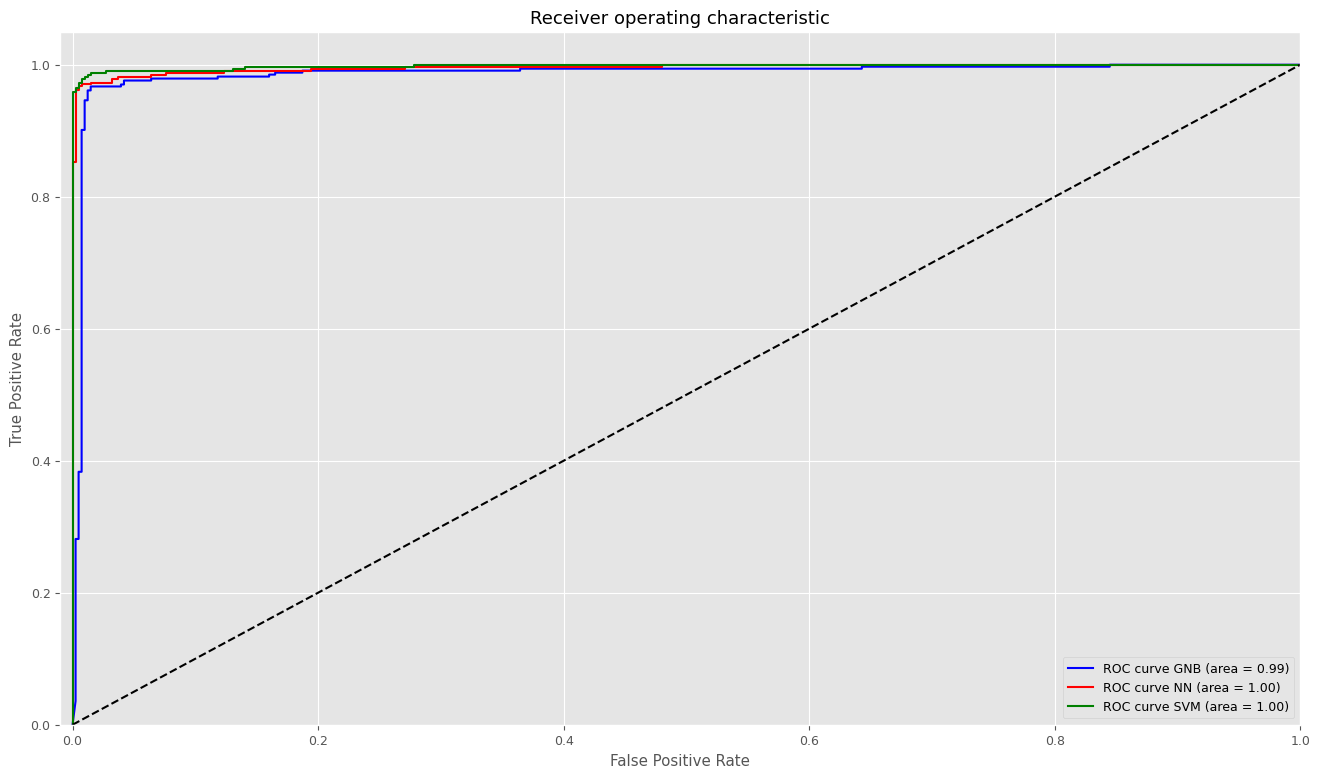
\includegraphics[width=\textwidth]{img/ris/roc_curve_corr.png}
    \caption{Curve ROC per i modelli addestrati su \texttt{dataset\_corr} e \texttt{dataset\_corr\_std}}
    \label{fig:roc_curve_corr}
\end{figure}

Le curve ROC permettono di confrontare i modelli addestrati anche con il classificatore
casuale, il quale corrisponde alla retta $y = x$. Il grafico riportato in figura
\ref{fig:roc_curve_corr} mostra che la rete neurale e il Gaussian Naive Bayes
hanno delle prestazioni molto simili tra loro, è quindi utile confrontare i due
due tramite l'area sottesa alla curva ROC (AUC). L'area sotto la curva ROC
per la rete neurale è pari a $1.00$, mentre per il Gaussian Naive Bayes è pari a
$0.99$. Questi valori suggeriscono che la rete neurale è leggermente superiore
al Gaussian Naive Bayes in termini di capacità di discriminazione tra le due
classi, anche se entrambi i modelli ottengono dei buoni risultati.

Come anticipato precedentemnte, dal momento che il dataset è di medie dimensioni
allora si è deciso di effettuare anche uno studio di robustezza dei modelli.
Per fare ciò si è deciso di condurre una valutazione tramite la tecnica della
$10$-fold stratified cross validation. Tale tecnica permette di ottenere una
stima più accurata delle performance del modello, riducendo l'effetto della
variabilità dei dati.

In questo processo ogni modello che è stato addestrato è stato valutato attraverso
le metriche di Accuracy, Precision, Recall e F1-score. I risultati ottenuti
dall'esecuzione della cross validation sono stati utilizzati per calcolare gli
intervalli di confidenza al $90\%$ delle metriche sopracitate.

Per svolgere questa operazione sono stati utilizzati \texttt{dataset\_corr} e 
\texttt{dataset\_corr\_std} completo, ovvero senza alcuna suddivisione in training 
set e test set.

I risultati ottenuti sono stati riportati sia in forma numerica che grafica
per facilitare la comprensione. In particolare, i valori delle metriche ottenuti
sono stati riportati in figura \ref{fig:intervalli_confidenza_corr} e
nella tabella \ref{tab:intervalli_confidenza_corr}.

\begin{table}[!ht]
    \begin{subtable}[h]{1\textwidth}
        \centering
        \begin{tabular}{@{}cllll@{}}
            \toprule
            \rowcolor[HTML]{EFEFEF}
            \textbf{Modello}                                      & \textbf{Accuracy}         & \textbf{Precision}          & \textbf{Recall}            & \textbf{F1-score}            \\ \midrule
            \cellcolor[HTML]{EFEFEF}\textbf{SVM}                  & \multicolumn{1}{c}{0 \%}     & \multicolumn{1}{c}{0 \%}     & \multicolumn{1}{c}{0 \%}     & \multicolumn{1}{c}{0 \%}     \\
            \cellcolor[HTML]{EFEFEF}\textbf{Gaussian Naive Bayes} & \multicolumn{1}{c}{95 \%}    & \multicolumn{1}{c}{90 \%}    & \multicolumn{1}{c}{99 \%}    & \multicolumn{1}{c}{94 \%}    \\
            \cellcolor[HTML]{EFEFEF}\textbf{Rete neurale}         & \multicolumn{1}{c}{98.27 \%} & \multicolumn{1}{c}{97.99 \%} & \multicolumn{1}{c}{98.15 \%} & \multicolumn{1}{c}{98.06 \%} \\ \bottomrule
        \end{tabular}
        \caption{Valore medio delle metriche ottenute dalla cross validation}
        \label{tab:risultati_cross_val_corr}
    \end{subtable}
    \hfill
    \begin{subtable}[h]{1\textwidth}
        \centering
        \begin{tabular}{@{}cllll@{}}
            \toprule
            \rowcolor[HTML]{EFEFEF}
            \textbf{Modello}                                      & \textbf{Accuracy} & \textbf{Precision} & \textbf{Recall}  & \textbf{F1-score}  \\ \midrule
            \cellcolor[HTML]{EFEFEF}\textbf{SVM}                  & []                   & []                  & []                 & []                 \\
            \cellcolor[HTML]{EFEFEF}\textbf{Gaussian Naive Bayes} & []                   & []                  & []                 & []                 \\
            \cellcolor[HTML]{EFEFEF}\textbf{Rete neurale}         & [97.98\%, 98.55\%]   & [97.47\%, 98.52\%]  & [97.49\%, 98.81\%] & [97.75\%, 98.38\%] \\ \bottomrule
        \end{tabular}
        \caption{Intervalli di confidenza delle metriche ottenute dalla cross validation}
        \label{tab:intervalli_confidenza_corr}
    \end{subtable}
    \caption{Risultati ottenuti dalla cross validation}
    \label{tab:intervalli_confidenza_corr}
\end{table}
% TODO: cambiare le immagini con quelle nuove
\begin{figure}[!ht]
    \centering
    \begin{subfigure}[b]{0.4\textwidth}
        \centering
        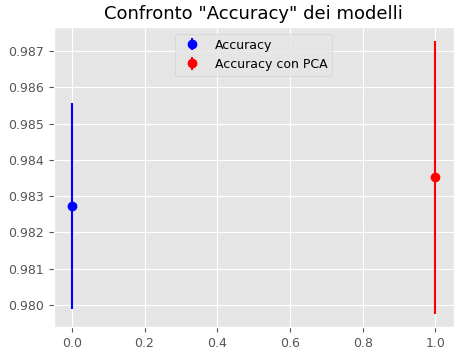
\includegraphics[width=\textwidth]{img/rete/intervalliAcc.png}
        \caption{Accuracy}
        \label{fig:acc}
    \end{subfigure}
    \hfill
    \begin{subfigure}[b]{0.4\textwidth}
        \centering
        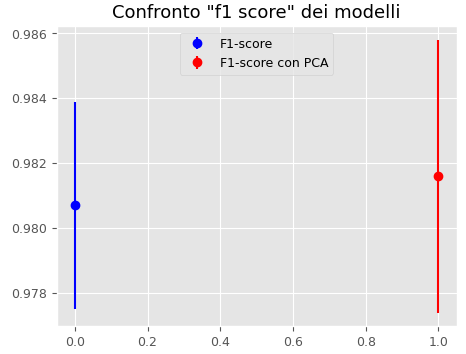
\includegraphics[width=\textwidth]{img/rete/intervalliF1.png}
        \caption{F1 score}
        \label{fig:f1}
    \end{subfigure}
    \hfill
    \begin{subfigure}[b]{0.4\textwidth}
        \centering
        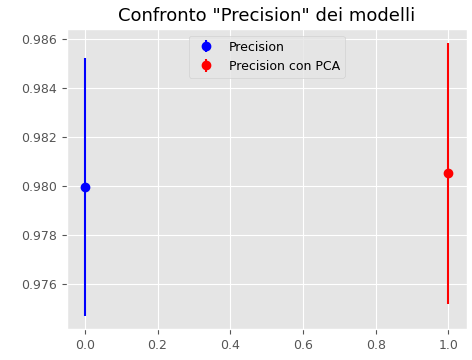
\includegraphics[width=\textwidth]{img/rete/intervalliPrecision.png}
        \caption{Precision}
        \label{fig:precision}
    \end{subfigure}
    \hfill
    \begin{subfigure}[b]{0.4\textwidth}
        \centering
        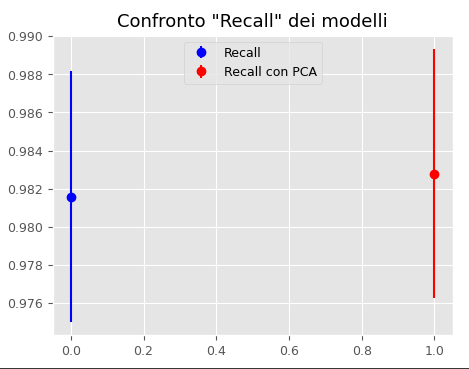
\includegraphics[width=\textwidth]{img/rete/intervalliRecall.png}
        \caption{Recall}
        \label{fig:recall}
    \end{subfigure}
    \caption{Intervalli di confidenza ottenuti dai modelli addestrati con e senza PCA}
    \label{fig:intervalli_confidenza_corr}
\end{figure}

% ! Commento sugli intervalli di confidenza e confronto con i valori ottenuti

\section{Risultati dei modelli allenati su \texttt{dataset\_pca} e \texttt{dataset\_pca\_std}} \label{sec:risultati_pca}
Un ragionamento analogo a quello svolto nella sezione \ref{sec:risultati_corr} può essere
applicato ai modelli addestrati sul dataset le cui feature sono state selezionate
attraverso Principal Component Analysis (PCA). 

Come prima cosa, nella figura \ref{fig:matrice_di_confusione_per_pca} vengono
mostrate le matrici di confusione dei modelli.

\begin{figure}[!ht]
    \centering
    \begin{subfigure}{0.45\textwidth}
        \centering
        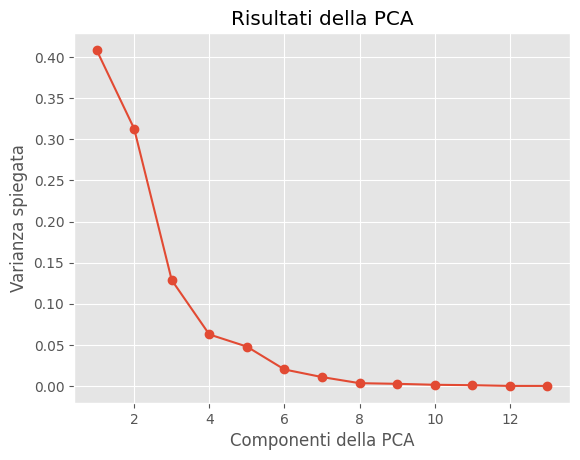
\includegraphics[width=\textwidth]{img/analisi/pcaVarianza.png}
        \caption{Support Vector Machine}
        \label{fig:matrice_di_confusione_per_SVM_pca}
    \end{subfigure}
    \hfill
    \begin{subfigure}{.45\textwidth}
        \centering
        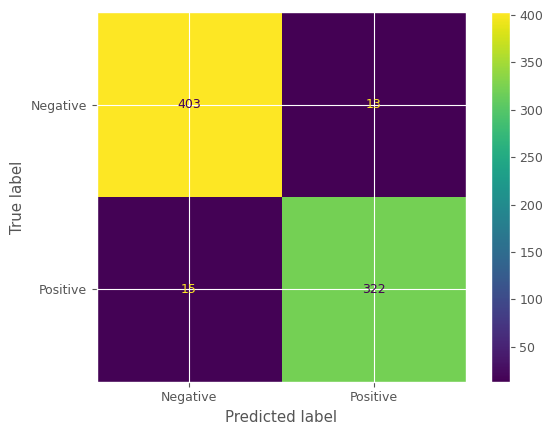
\includegraphics[width=\textwidth]{img/gnb/confusion_matrix_pca.png}
        \caption{Gaussian Naive Bayes}
        \label{fig:matrice_di_confusione_per_GNB_pca}
    \end{subfigure}
    \hfill
    \begin{subfigure}{.45\textwidth}
        \centering
        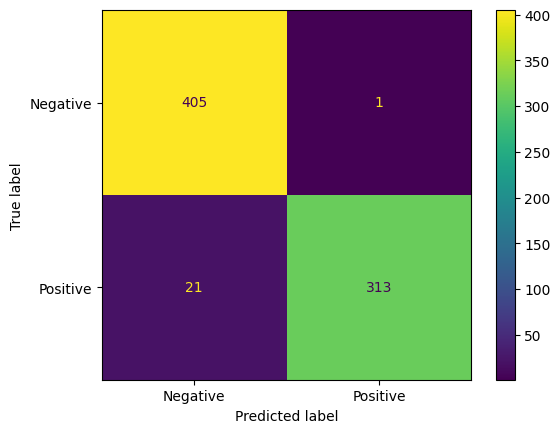
\includegraphics[width=\textwidth]{img/rete/matrice_confusione_PCA.png}
        \caption{Rete neurale}
        \label{fig:matrice_di_confusione_per_NN_pca}
    \end{subfigure}
    \caption{Matrici di confusione per i modelli addestrati su \texttt{dataset\_pca} e \texttt{dataset\_pca\_std}}
    \label{fig:matrice_di_confusione_per_pca}
\end{figure}

Successivamente sono state ricavate dalle matrici di correlazione le metriche 
di valutazioen dei vari modelli, i valori sono riportati nella tabella 
\ref{tab:risultati_pca}.

\begin{table}[!ht]
    \centering
    \begin{tabular}{@{}cllll@{}}
        \toprule
        \rowcolor[HTML]{EFEFEF}
        \textbf{Modello}                                      & \textbf{Accuracy}         & \textbf{Precision}          & \textbf{Recall}            & \textbf{F1-score}            \\ \midrule
        \cellcolor[HTML]{EFEFEF}\textbf{SVM}                  & \multicolumn{1}{c}{0 \%}     & \multicolumn{1}{c}{0 \%}     & \multicolumn{1}{c}{0 \%}     & \multicolumn{1}{c}{0 \%}     \\
        \cellcolor[HTML]{EFEFEF}\textbf{Gaussian Naive Bayes} & \multicolumn{1}{c}{96 \%}    & \multicolumn{1}{c}{96 \%}    & \multicolumn{1}{c}{96 \%}    & \multicolumn{1}{c}{96 \%}    \\
        \cellcolor[HTML]{EFEFEF}\textbf{Rete neurale}         & \multicolumn{1}{c}{98.27 \%} & \multicolumn{1}{c}{97.92 \%} & \multicolumn{1}{c}{98.21 \%} & \multicolumn{1}{c}{98.07 \%} \\ \bottomrule
    \end{tabular}
    \caption{Risultati ottenuti dal modello addestrato}
    \label{tab:risultati_pca}
\end{table}

I risultati ottenuti rivelano prestazioni molto simili con quelle ottenute per il
dataset le cui feature sono state selezionate manualmente.

Inoltre, anche in questo caso, è possibile confrontare i modelli attraverso le curve
ROC, le quali sono riportate in figura \ref{fig:roc_curve_pca}.
\begin{figure}[!ht]
    \centering
    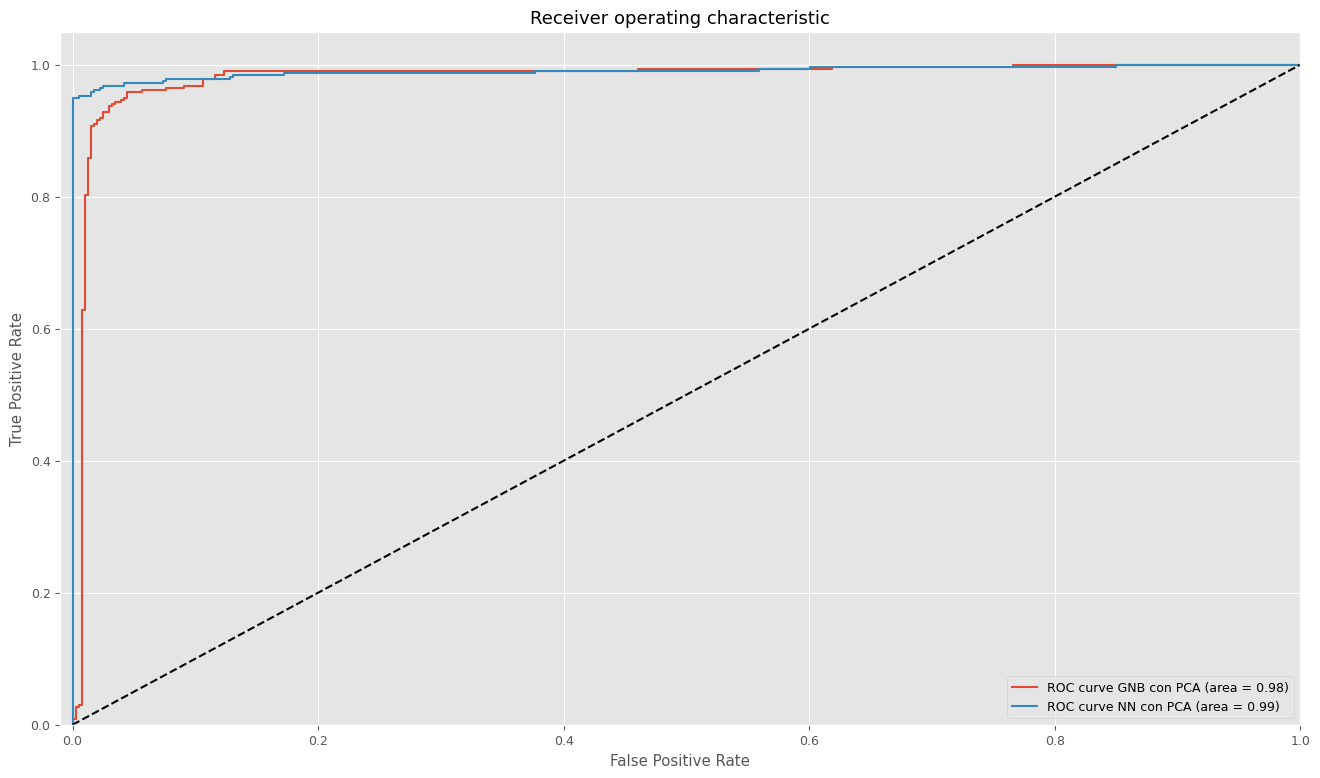
\includegraphics[width=\textwidth]{img/ris/roc_curve_pca.png}
    \caption{Curve ROC per i modelli addestrati su \texttt{dataset\_pca} e \texttt{dataset\_pca\_std}}
    \label{fig:roc_curve_pca}
\end{figure}

Utilizzando la PCA per la creazione del dataset nelle curve ROC si può notare
una maggiore distanza tra la curva ROC della rete neurale e quella del Gaussian
Naive Bayes. Inoltre, calcolando l'area sotto la curva ROC (AUC) si può notare
come la rete neurale sia leggermente superiore al Gaussian Naive Bayes, con un
valore di $0.99$ per la rete neurale e di $0.98$ per il Gaussian Naive Bayes. Il
che suggerisce che questi classificatori sono leggermente peggiori rispetto a
quelli addestrati sul dataset le cui feature sono state selezionate manualmente.

Infine, per restare coerenti con quanto fatto in precedenza, è possibile effettuare
una valutazioen di robustezza dei modelli addestrati tramite la tecnica della 
$10$-fold stratified cross validation. 
I risultati ottenuti sono riportati in figura \ref{fig:intervalli_confidenza_pca}
e nella tabella \ref{tab:intervalli_confidenza_pca}.

\begin{table}[!ht]
    \begin{subtable}[h]{1\textwidth}
        \centering
        \begin{tabular}{@{}cllll@{}}
            \toprule
            \rowcolor[HTML]{EFEFEF}
            \textbf{Modello}                                      & \textbf{Accuratezza}         & \textbf{Precisione}          & \textbf{Richiamo}            & \textbf{F1 score}            \\ \midrule
            \cellcolor[HTML]{EFEFEF}\textbf{SVM}                  & \multicolumn{1}{c}{0 \%}     & \multicolumn{1}{c}{0 \%}     & \multicolumn{1}{c}{0 \%}     & \multicolumn{1}{c}{0 \%}     \\
            \cellcolor[HTML]{EFEFEF}\textbf{Gaussian Naive Bayes} & \multicolumn{1}{c}{96 \%}    & \multicolumn{1}{c}{96 \%}    & \multicolumn{1}{c}{96 \%}    & \multicolumn{1}{c}{96 \%}    \\
            \cellcolor[HTML]{EFEFEF}\textbf{Rete neurale}         & \multicolumn{1}{c}{98.35 \%} & \multicolumn{1}{c}{98.05 \%} & \multicolumn{1}{c}{98.27 \%} & \multicolumn{1}{c}{98.15 \%} \\ \bottomrule
        \end{tabular}
        \caption{Valore medio delle metriche ottenute dalla cross validation}
        \label{tab:risultati_cross_val_pca}
    \end{subtable}
    \hfill
    \begin{subtable}[h]{1\textwidth}
        \centering
        \begin{tabular}{@{}cllll@{}}
            \toprule
            \rowcolor[HTML]{EFEFEF}
            \textbf{Modello}                                      & \textbf{Accuratezza} & \textbf{Precisione} & \textbf{Richiamo}  & \textbf{F1 score}  \\ \midrule
            \cellcolor[HTML]{EFEFEF}\textbf{SVM}                  & []                   & []                  & []                 & []                 \\
            \cellcolor[HTML]{EFEFEF}\textbf{Gaussian Naive Bayes} & []                   & []                  & []                 & []                 \\
            \cellcolor[HTML]{EFEFEF}\textbf{Rete neurale}         & [97.97\%, 98.72\%]   & [97.51\%, 98.58\%]  & [97.62\%, 98.93\%] & [97.73\%, 98.58\%] \\ \bottomrule
        \end{tabular}
        \caption{Intervalli di confidenza delle metriche ottenute dalla cross validation}
        \label{tab:intervalli_confidenza_pca}
    \end{subtable}
    \caption{Risultati ottenuti dalla cross validation}
    \label{tab:intervalli_confidenza_pca}
\end{table}

% TODO: Sono da calcolare e inserire
\begin{figure}[!ht]
    \centering
    \begin{subfigure}[b]{0.4\textwidth}
        \centering
        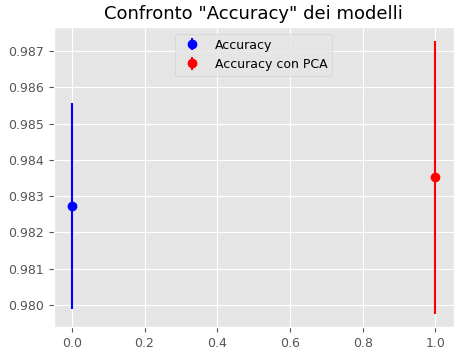
\includegraphics[width=\textwidth]{img/rete/intervalliAcc.png}
        \caption{Accuracy}
        \label{fig:acc_pca}
    \end{subfigure}
    \hfill
    \begin{subfigure}[b]{0.4\textwidth}
        \centering
        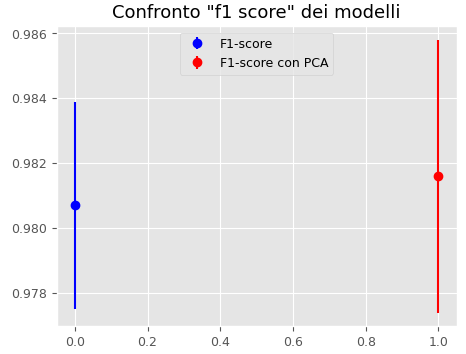
\includegraphics[width=\textwidth]{img/rete/intervalliF1.png}
        \caption{F1 score}
        \label{fig:f1_pca}
    \end{subfigure}
    \hfill
    \begin{subfigure}[b]{0.4\textwidth}
        \centering
        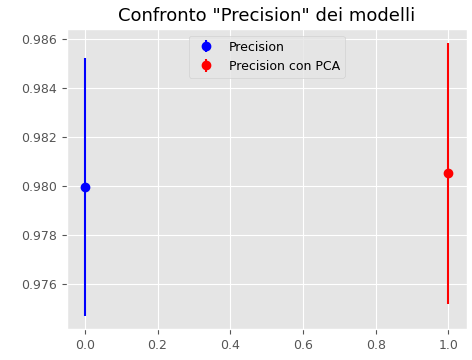
\includegraphics[width=\textwidth]{img/rete/intervalliPrecision.png}
        \caption{Precision}
        \label{fig:precision_pca}
    \end{subfigure}
    \hfill
    \begin{subfigure}[b]{0.4\textwidth}
        \centering
        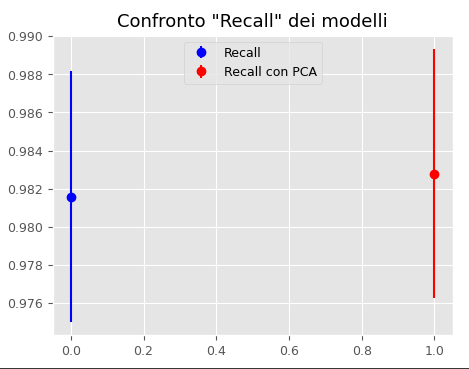
\includegraphics[width=\textwidth]{img/rete/intervalliRecall.png}
        \caption{Recall}
        \label{fig:recall_pca}
    \end{subfigure}
    \caption{Intervalli di confidenza ottenuti dai modelli addestrati con e senza PCA}
    \label{fig:intervalli_confidenza_pca}
\end{figure}

% ! Commento dei risultati da fare